\documentclass[12pt,letterpaper]{article}
\usepackage{dirtytalk}
\usepackage{preamble}

\newcommand\course{CSCI 544}
\newcommand\hwnumber{}
\newcommand\userID{Kathleen Xue, Jianxing Ke, \\  Guohao Li, Yichen Wu}
\begin{document}
\section*{Submission} We chose to use Github to submit our code. \href{https://github.com/kathleen-xue/csci544project}{Here} is the repository. The students who worked on this project were Kathleen Xue (kxue@usc.edu, SID 6824587964), Jianxing Ke (jianxink@usc.edu, SID 7285185934), Guohao Li (guohaol@usc.edu, SID 2912331182), and Yichen Wu (wuyichen@usc.edu, SID 8106714357). 
\section*{a. Task Description, Problem Formulation}
The task we decided to complete for this course project was Natural Language Inference, a task in which the model tries to determine whether a hypothesis is true, false, or undetermined given a premise. The way this problem is formulated is as a classification problem, where each hypothesis is classified as neutral, contradiction, or entailment based on the premise. For instance, the following table gives a good example of the natural language inference task and classifying hypotheses.
\begin{center}
    \begin{tabular}{| c | c | c |}
        \hline
        \textbf{Text} & \textbf{Judgment} & \textbf{Hypothesis} \\ \hline
        A woman walks into the department store. & contradiction & The woman is sleeping.
        \\ \hline
        A girl is eating ice cream. & neutral & Two girls are talking and eating. \\ \hline
        A lady meets up with her friends. & contradiction & The lady is by herself. \\ \hline
        Two men argue about stocks & entailment & The men are talking. \\ \hline
    \end{tabular}
\end{center}
\section*{b. Baseline Algorithm}
The baseline algorithm our group decided to use for this task was the Bowman model, which is a simple lexicalized classifier that implements 6 features types: 
\begin{enumerate}
    \item BLEU score of the hypothesis in comparison with the premise (with n-gram length between 1 and 4)
    \item Difference in length between hypothesis and premise
    \item Amount of overlap between the words used in the hypothesis and the words used in the premise
    \item An indicator for every unigram and bigram in the hypothesis
    \item Indicators for cross-unigrams between the premise and the hypothesis
    \item Indicators for cross-bigrams between the premise and the hypothesis
\end{enumerate}
The reason we chose to use a simple lexicalized classifier is because it actually performs quite well on the SNLI dataset, which is also used for our improved algorithm (in the Bowman paper, the lexicalized classifier was able to correctly classify 78 percent of the test dataset). 
\section*{c. Approach}
In our approach, we decided to take inspiration from the paper DR-BiLSTM: Dependent Reading BiLSTM for Natural Language Inference by Reza Ghaeini et al.  The DR-BiLSTM model has four major components: input encoding, attention, inference, and finally classification.  \\ \\ 
In terms of input encoding, because RNNs are commonly used in this step, the paper chose to utilize a bidirectional LSTM to complete this. The intuition for using the bidirectional LSTM instead of RNN is that this encoding method gives a more informative encoding by taking into account the history of both the premise and the hypothesis, which an RNN is incapable of doing. \\ \\ 
In the attention step of the model, the paper utilizes a soft-alignment to connect relevant sub-components between the premise and the hypothesis. We then take these vectors and concatenate them with the difference and element-wise product vectors, before feeding them into a feed-forward neural layer with a ReLU activation function. \\ \\
During the inference step of the model, the paper chooses to use another bidirectional LSTM to combine the two vectors computed from the attention step. The bidirectional LSTM is similar to the one used in the encoding step, but instead of only using dependent reading information, the inference steps passes in both dependent reading information as well as independent reading information into a max-pooling layer (which allows us to maximize the inferencing ability of the model because we now consider both independent and dependent readings). \\ \\
In classification, the final step of the model, the paper takes the vectors aggregated from the inference stage and feeds them into a multilayer perceptron classifier with a tanh activation and softmax output layer. \\ \\
Our group decided to build this model from end to end in order to replicate its results and see for ourselves the improvement that this model has on natural language inference as compared with a simple lexicalized classifier. We used boilerplate preprocessing, embedding, and training code from Github user Aurelien Coet's   \href{https://github.com/coetaur0/LEAN}{repository}. All the final results of both models can be viewed in our team's project \href{https://github.com/kathleen-xue/csci544project}{repository}.
\section*{d. Results Analysis}
We found from running both the baseline algorithm and the paper algorithm on training and test datasets that the paper algorithm achieved a significantly higher accuracy than the baseline algorithm. The below table compares the training and validation accuracies of the paper algorithm (with both the preset hyperparameters and with some hyperparameter tuning) with the training and validation accuracies of the baseline algorithm. 
\begin{center}
    \begin{tabular}{| c | c | c |}
        \hline
         & \textbf{Training} & \textbf{Validation}\\ \hline
        \textbf{Bowman model} & 66.10$\%$ & 64.90$\%$
        \\ \hline
        \textbf{DR-BiLSTM model (preset hyperparameters)*} & 90.81$\%$ & 87.18$\%$\\ \hline
        \textbf{DR-BiLSTM model (with batch=64)} & 89.29$\%$ & 87.07$\%$\\ \hline
    \end{tabular} \\
    * hidden=450, batch=32, learning rate=0.0004, dropout=0.4 \\
\end{center}
Moreover, looking at the cross-entropy loss over multiple epochs, we can immediately tell that the cross entropy loss in the paper algorithm becomes lower earlier than the cross entropy loss of the baseline algorithm. \\
\\
As seen below, the cross-entropy loss of the Bowman model (left graph) approaches a minimum of around 0.60 after 50 epochs, but the DR-BiLSTM cross entropy loss (right graph) hits a minimum of around 0.25 after only 5 epochs. This means that the DR-BiLSTM model has a lower cross entropy loss, or a lower divergance between predicted judgments and actual judgments, than the Bowman model.\\
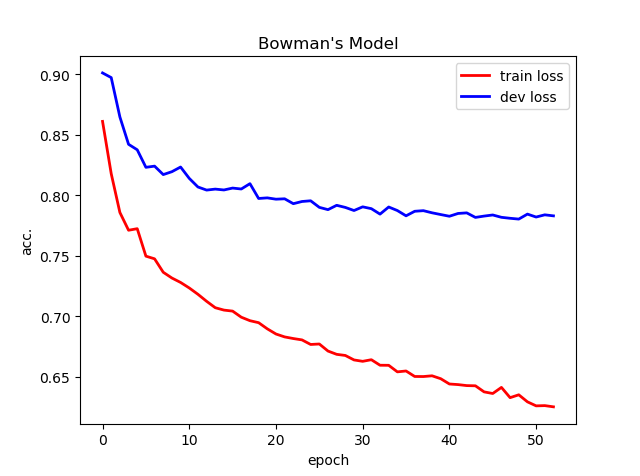
\includegraphics[scale=0.53]{Bowmanxent.PNG}
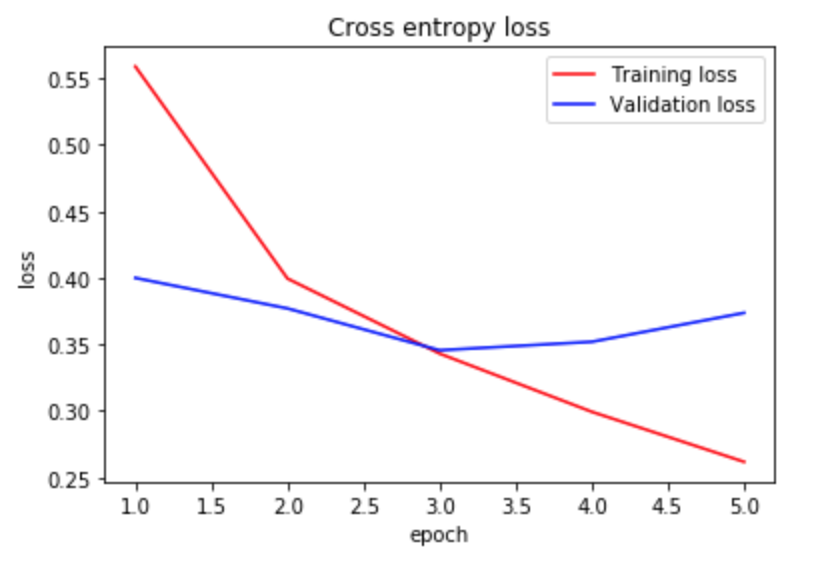
\includegraphics[scale=0.58]{DRLSTMxent.png} \\
\\
Beyond basic analyses, our group decided to analyze other more specific features of the model to understand the DR-BiLSTM and Bowman models' \say{rationales} better. We decided to analyze results based on three types of features: overlap between premise and hypothesis, sentence length, and whether the sentence contains specific types of words (we chose to analyze based on whether the sentence contains negation, quantifier, and belief words). The following table displays the results we obtained by dividing the model results by feature. \\ \\
In terms of overlap, we defined a premise and hypothesis pair as having high overlap if the sentences share more than 70$\%$ of tokens; regular overlap if the sentences share between 30 and 70$\%$ tokens; and low overlap if the sentences share fewer than 30$\%$ of tokens. \\ \\ 
In terms of sentence length, we defined a premise and hypothesis pair as being long if either sentence contains more than 20 tokens; regular if either sentence is between 5 and 20 tokens; and short if either sentence is fewer than 5 tokens. \\ \\
For negation, we constructed a negation set from an online dictionary: $\{$no, not, none, no one, nobody, nothing, neither, nowhere, never, hardly, scarcely, barely, doesn’t, isn’t, wasn’t, shouldn’t, wouldn’t, couldn’t, won’t, can’t, don’t$\}$. If either of the sentences contains any of the words in the negation set, we defined the premise-hypothesis pair as containing negation. The same was done for quantifiers and beliefs; for quantifiers, we used the set $\{$much, enough, more, most, less, least, no, none,
some, any, many, few, several, almost, nearly$\}$; for beliefs, we used the set $\{$know, believe,
understand, doubt, think, suppose, recognize,
forget, remember, imagine, mean, agree, disagree, deny, promise$\}$. \\ \\
Surprisingly, the Bowman model did poorly with high-overlap sentences while the DR-BiLSTM model did well on that exact same category. This might be because the Bowman model does not take into account sequence for sentences, and may in fact have missed some key semantic details that the DR-BiLSTM model was able to catch for these high-overlap sentences. Another surprising result from the below accuracies is the high performance of the Bowman model on sentences that contain belief words. We are unsure of why this might be, and think that this could be an area where we might want to think about conducting further experiments if we were to expand this project. 
\begin{center}
    \begin{tabular}{| c | c | c |} \hline
         &  \textbf{Bowman} & \textbf{DR-BiLSTM} \\
         \hline
        \textbf{Overlap: High} & 0.57 & 0.92 \\ 
        \hline
        \textbf{Overlap: Reg} & 0.63 & 0.88 \\
        \hline
        \textbf{Overlap: Low} & 0.66 & 0.86 \\
        \hline
        \textbf{Length: Long} & 0.66 & 0.86 \\
        \hline
        \textbf{Length: Reg} & 0.65 & 0.87 \\
        \hline
        \textbf{Length: Short} & 0.64 & 0.90 \\
        \hline
        \textbf{Contains Negation} & 0.74 & 0.88 \\
        \hline
        \textbf{Contains Quantifier} & 0.67 & 0.85 \\
        \hline
        \textbf{Contains Belief} & 0.86 & 0.86 \\
        \hline
    \end{tabular}
\end{center}
We then looked at accuracy based on label, and found the test accuracy results displayed in the following table. 
\begin{center}
    \begin{tabular}{|c|c|c|} \hline
         &  \textbf{Bowman} & \textbf{DR-BiLSTM}\\
         \hline
        \textbf{Entailment Accuracy} & 0.68 & 0.89 \\
        \hline
        \textbf{Neutral Accuracy} & 0.68 & 0.81 \\
        \hline
        \textbf{Contradiction Accuracy} & 0.58 & 0.90 \\
        \hline
    \end{tabular}
\end{center}
We expected both models' neutral statement accuracies were consistently lower than their entailment and contradiction statement accuracies, but according to the table above the Bowman model actually performed better on neutral hypotheses than on contradiction hypotheses. Because this seemed counterintuitive, we wanted to further delve into how the two models might be labeling neutral as opposed to entailment and contradiction hypotheses. First, we took the DR-BiLSTM's predicted softmax probabilities and plotted them on a 3D graph to better visualize the model's perspective of each of the three labels.\\ \\
We can interpret each of the datapoints in the graphs below as how much the DR-BiLSTM model is \say{leaning} toward each of the labels. This is possible because the output probabilities are gotten from a softmax layer, which weights the probabilities and has the property that the sum of the probabilities sum to 1. So, for instance, given a datapoint [0.1, 0.2, 0.7] (where index i indicates the predicted probability that the hypothesis is of label i, and index 0=Entailment, index 1=Neutral, and index 2=Contradiction), when this datapoint is plotted onto the graph, we can see that the datapoint is majority-weighted in contradiction. \\ \\ 
As such, we can easily tell from the graphs below that for ground truth entailment and contradiction hypotheses, the model very heavily leans toward the correct labels. For entailment and contradiction, in fact, the model very clearly knows that a ground truth entailment hypothesis is not a contradiction hypothesis, and vice-versa. But for ground truth neutral hypotheses, the model is actually visibly \say{confused} and has heavy collections of datapoints leaning towards both entailment and contradiction, meaning that the model in general can discern a neutral hypothesis correctly, but that the model sees the neutral hypothesis as close to both entailment and contradiction.
\begin{center}
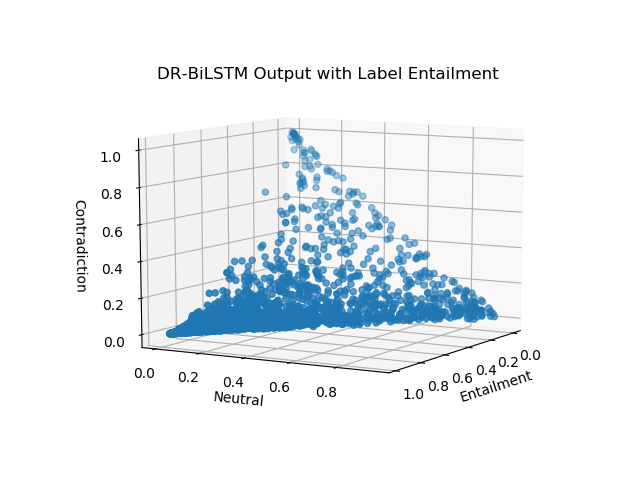
\includegraphics[scale=0.35]{lstmEntailment.png}
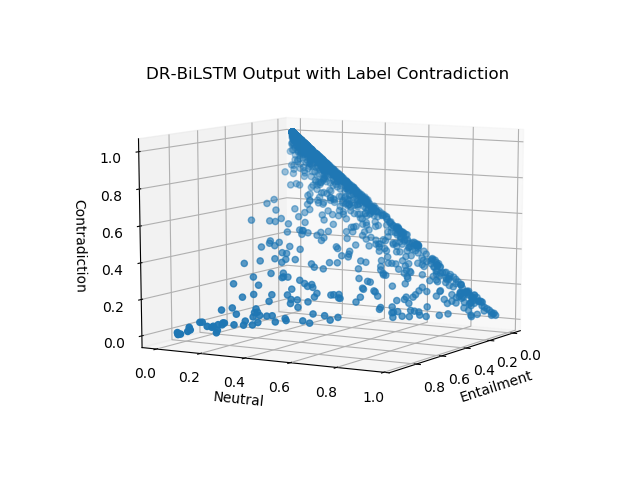
\includegraphics[scale=0.35]{lstmContradiction.png}
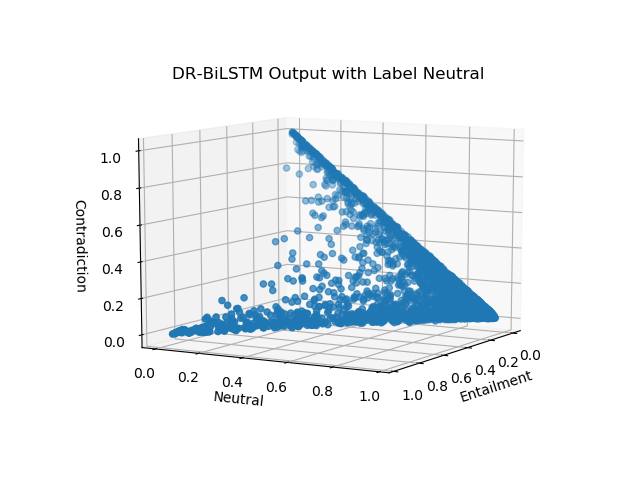
\includegraphics[scale=0.35]{lstmNeutral.png}
\end{center}\\
Contrasting the DR-BiLSTM model with the Bowman model, it becomes immediately clear that the DR-BiLSTM model's output probabilities are far more certain than the probabilities outputted by the Bowman model. Although the Bowman model only performs on average about 20$\%$ worse than the DR-BiLSTM model, the output probabilities it generates from its softmax layer have more noise, as we can see from the fact that the datapoints in the graphs below are not clustered tightly near the ground truth label but are rather clustered more generally around the ground truth label. Whereas for the DR-BiLSTM model it is much more clear-cut if a hypothesis belongs to entailment as opposed to contradiction, for the Bowman model each label is a fuzzy region and the Bowman model does not seem to see the neutral label as a middle ground between entailment and contradiction as the DR-BiLSTM model does.
\begin{center}
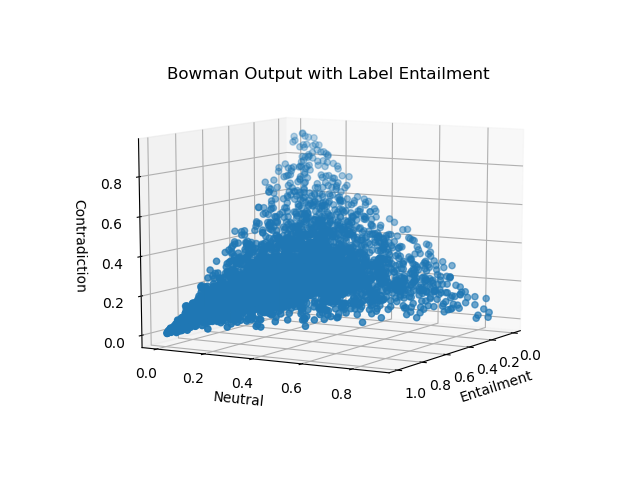
\includegraphics[scale=0.35]{bowmanEntailment.png}
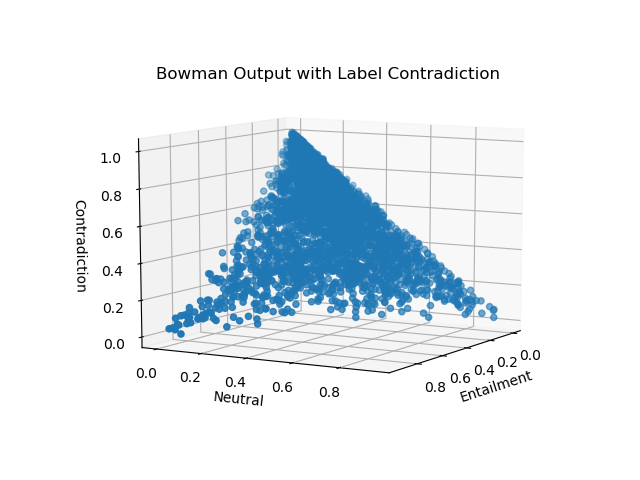
\includegraphics[scale=0.35]{bowmanContradiction.png}
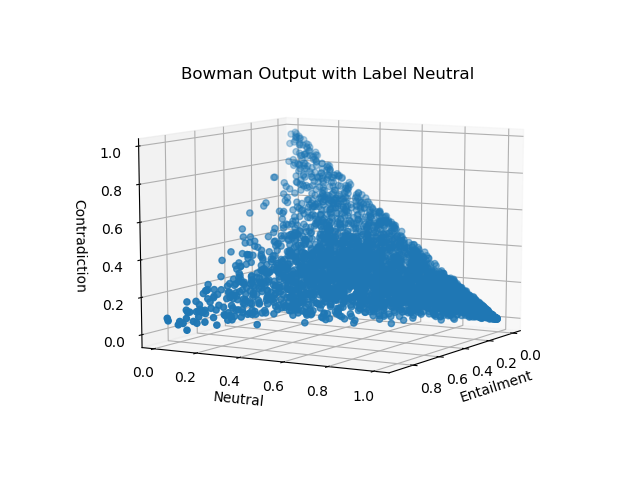
\includegraphics[scale=0.35]{bowmanNeutral.png}
\end{center}
\section*{e. Qualitative Analysis}
Given a list of test sentences from the SNLI test dataset (below), we ran both the Bowman model and the DR-BiLSTM model on these five sentences and outputted their labels as compared with the ground truth. \\
\begin{enumerate}
    \item 
    \textbf{Text:} This church choir sings to the masses as they sing joyous songs from the book at a church. \\
    \textbf{Hypothesis:} The church has cracks in the ceiling.
    \item
    \textbf{Text:} This church choir sings to the masses as they sing joyous songs from the book at a church. \\
    \textbf{Hypothesis:} The church is filled with song. 
    \item 
    \textbf{Text:} This church choir sings to the masses as they sing joyous songs from the book at a church. \\
    \textbf{Hypothesis:} A choir singing at a baseball game.
    \item 
    \textbf{Text:} A woman with a green headscarf, blue shirt and a very big grin. \\
    \textbf{Hypothesis:} The woman is young.
    \item
    \textbf{Text:} A woman with a green headscarf, blue shirt and a very big grin. \\
    \textbf{Hypothesis:} The woman is very happy.
\end{enumerate}
The following table displays the 5 judgments each model made along with the ground truth judgments.
\begin{center}
    \begin{tabular}{|c|c|c|c|c|c|}
         \hline
         &  \textbf{1} & \textbf{2} & \textbf{3} & \textbf{4} & \textbf{5} \\ \hline
        \textbf{Ground truth} & Neutral & Entailment & Contradiction & Neutral & Entailment \\ \hline
        \textbf{Bowman} & Contradiction & Contradiction & Contradiction & Neutral & Neutral \\ \hline
        \textbf{DR-BiLSTM} & Contradiction & Entailment & Contradiction & Neutral & Neutral \\ \hline
    \end{tabular}
\end{center}
The DR-BiLSTM model predicted 3 labels correctly out of 5 examples. The judgment for the first sentence should be neutral, while the model predicted contradiction; the judgment for the last sentence should be entailment, while the model predicted neutral. The Bowman model, on the other hand, predicted 2 labels correctly out of 5 examples. Both models predicted correctly for the third and the fourth pairs; both models predicted the incorrect \say{contradiction} for the first pair, and the incorrect “neutral” for the last pair. \\
\\
Perhaps the reason that both models incorrectly labeled the first sentence is that none of the words in the hypothesis are synonyms of the words in the text, but that the word \say{cracks} might be considered similar to the word \say{books} in some models. In terms of the last sentence, it is unclear why both models predicted the judgment would be neutral rather than entailment, as \say{happy} should be a very close synonym to \say{grin}. One factor that might have helped cause the models' incorrect judgments is that the models might not have assigned \say{a very big grin} to \say{a woman} because the given text is a phrase rather than a complete sentence. If the models failed to connect the fact that it was the woman who was grinning, then it makes sense that both of them saw the hypothesis of the woman being happy as neutral rather than entailment.
\end{document}